\documentclass[letterpaper, 11pt]{article} 

\usepackage{graphics,graphicx}
\usepackage{multicol} 
\usepackage{parskip}
\usepackage{amsmath}
\usepackage{multirow}
\usepackage[utf8]{inputenc}
\usepackage{fancyhdr}
\usepackage[title]{appendix}
\usepackage{wasysym}
\usepackage{url}
\usepackage{subcaption}

\usepackage[font=footnotesize,labelfont=small]{caption}
\captionsetup{width=0.85\linewidth}

\RequirePackage{geometry}
\geometry{margin=2cm}

\setlength{\parskip}{0.2cm}
\setlength{\parindent}{0pt}


\title{Preject 3 Report: Cache Replacement Policies on AI Workloads}
\author{
Tai Duc Nguyen \\
ECEC 412: Modern Processor Design
}
\date{\today}

\begin{document}

\maketitle
\rule{\textwidth}{1pt}

\begin{abstract}
	Cache is a solution to the problem of slow memory access in modern computer architecture. From the dawn of the 21st century, many CPU manufacturer, especially Intel and IBM has implemented combinations of advanced dynamic caching techniques, which can be divided into two categories: hardware and software. Some famous hardware techniques, which tackle the issues of maintaning efficient power management while providing fast cache access, are: multi-tiered cache levels and set-associative caching. However, software techniques provide the ability to increase cache hit rate. Some examples include way-predictions methods and cache replacement policies. In this project, different cache replacement policies: Least Recently Used (LRU) and Least Frequently Used (LFU) are evaluated performance wise with different hardware configurations: block size, cache size and number of associative sets.
\end{abstract}

\section{Introduction}
\label{intro}
	In order to achieve the objective of evaluating the performance of different cache replacement policies, a simulation was written in C by Shihao Song and Adarsha Balaji (available here: \url{https://github.com/Shihao-Song/Computer-Architecture-Teaching/tree/master/C621/Cache_Policy}). Using the framework established, a mechanism to test all pre-defined hardware configurations at once is written on top. After automating the testing of different configs, the LFU replacement policy is implemented in a similar fashion to the already existed code for the LRU replacement policy.

\section{Simulation and Results}
	From the procedures in Section \ref{intro}, a sample output from the output is shown in Figure \ref{fig1} below:
	
	\begin{figure}[htb!]
		\centering
		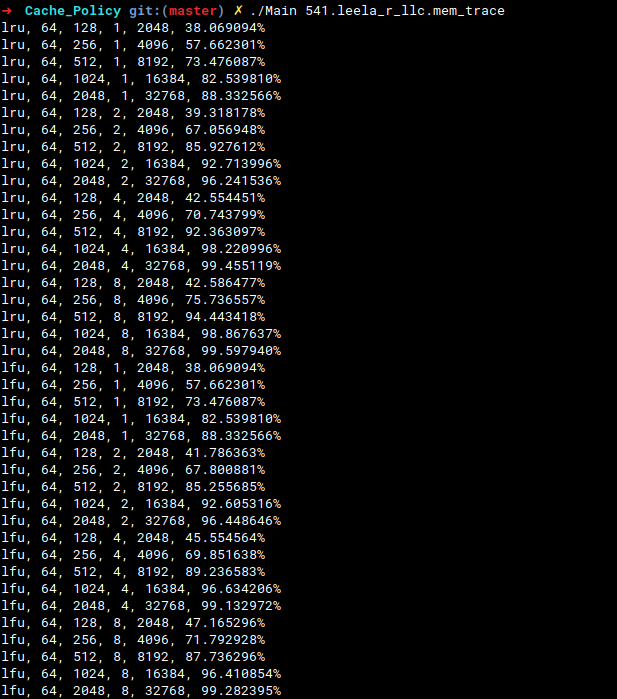
\includegraphics[width=0.5\linewidth]{sample_program_output.png}
		\caption{Sample output of the simulation}
		\label{fig1}
	\end{figure}

	The columns in the sample are respectively:
		\begin{itemize}
			\item Type of replacement policy
			\item Block size (in bytes)
			\item Cache size (in KB)
			\item Number of associative sets 
			\item Number of cache blocks
			\item Cache hit rate in percentage
		\end{itemize}
	
	Performing this simulation over all 3 memory traces (each trace includes many Load and Store instructions), the results are shown in graphs (Figure 2 \ref{fig2a}, \ref{fig2b}, \ref{fig2c}, and \ref{fig2d}).
	
	\newpage
	
	\begin{figure}[ht!]
		\centering
		\begin{subfigure}[b]{.48\linewidth}
			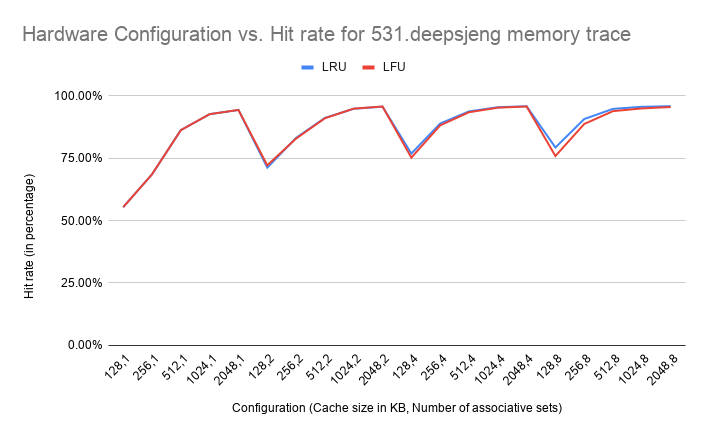
\includegraphics[width=\textwidth]{531_deepsjeng_results.png}
			\caption{Results for 531.deepsjeng memory trace}
			\label{fig2a}
		\end{subfigure}
%		\hskip2em
		\begin{subfigure}[b]{.48\linewidth}
			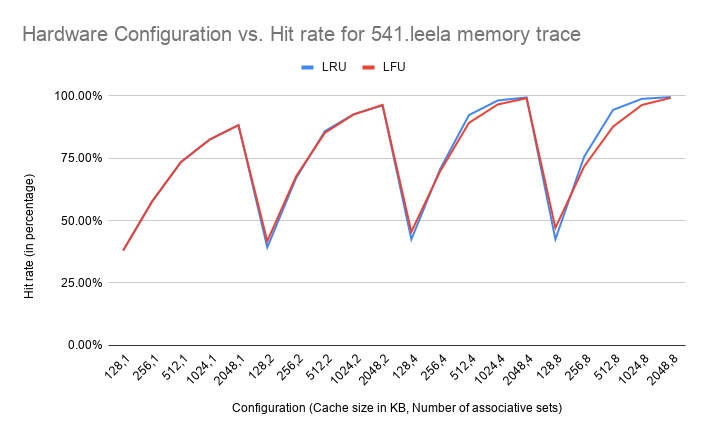
\includegraphics[width=\textwidth]{541_leela_results.png}
			\caption{Results for 541.leela memory trace}
			\label{fig2b}
		\end{subfigure}
		\begin{subfigure}[b]{.48\linewidth}
			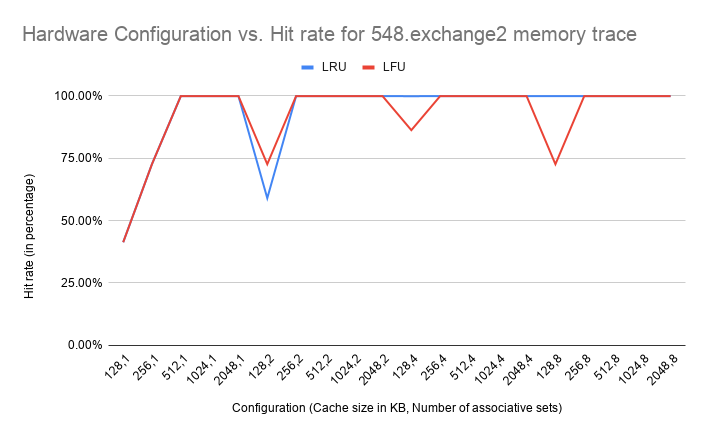
\includegraphics[width=\textwidth]{548_exchange2_results.png}
			\caption{Results for 548.exchange2 memory trace}
			\label{fig2c}
		\end{subfigure}
%		\hskip2em
		\begin{subfigure}[b]{.48\linewidth}
			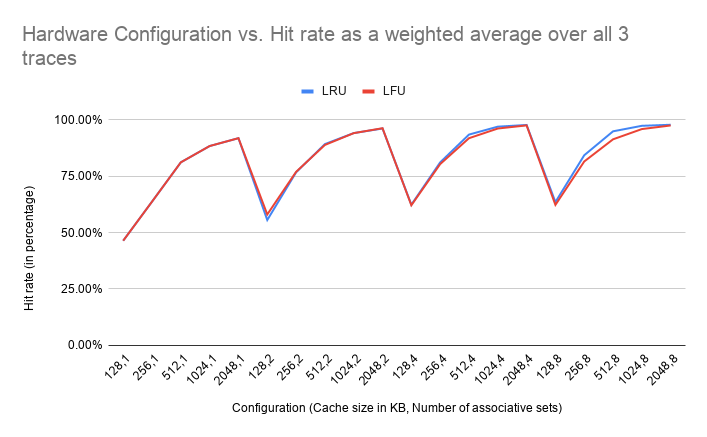
\includegraphics[width=\textwidth]{all_weighted_avg_results.png}
			\caption{Overall results as weighted averages of 3 traces}
			\label{fig2d}
		\end{subfigure}
		\caption{Simulation results. The x-axis have different hardware configurations with the first number being the cache size in KB and the second number being the number of associative sets. The y-axis is the cache hit rate in percentage.}
	\end{figure}
	
	From all the figures above, the general trend is that the hit rate increase when:
	\begin{itemize}
		\item The cache size increases
		\item The number of associative cache stores increases
	\end{itemize}

	Regarding the 2 different replacement policies, LFU does better than LRU only when the number of associative cache stores is small (1 or 2). LRU has higher hit rate than LFU with larger number of associative cache stores (4 or 8). This behavior is seen most clear from the results for the 548.exchange2 memory trace. It is noted that different memory traces have different number of instructions, hence, the overall performance of each policy is decided as a weighted average and shown in Figure \ref{fig2d}. 

\section{Discussion}
	From the results above, the fact that cache hit rate is directly proportional to cache size and number of associative cache stores is consistent with other literature on this subject. Also, from the data, it can also be shown that the increase in performance is not linear, but rather curving out, which means that there will be diminishing returns for large cache size and high number of associative cache due to limitation in hardware area and power consumption. 

\end{document}